\section*{7.2 带约束优化与拉格朗日乘子}
\addcontentsline{toc}{section}{7.2 带约束优化与拉格朗日乘子}
\label{sec:7.2}

在上一节中，我们考虑了求解函数极小值的问题：

\begin{equation}
\min_{\boldsymbol{x}} f(\boldsymbol{x})
\tag{7.16}\label{eq:7-16}
\end{equation}

其中 $ f : \mathbb{R}^D \to \mathbb{R} $。

在本节中，我们增加了额外的约束。也就是说，对于实值函数 $ g_i : \mathbb{R}^D \to \mathbb{R} $（$ i = 1, \ldots, m $），我们考虑如下带约束优化问题（见图~\ref{fig:7-4} 示意）：

\begin{equation}
\begin{aligned}
\min_{\boldsymbol{x}} & \quad f(\boldsymbol{x}) \\
\text{subject to} & \quad g_i(\boldsymbol{x}) \leqslant 0 \quad \textcn{对所有 } i = 1, \ldots, m \textcn{。}
\end{aligned}
\tag{7.17}\label{eq:7-17}
\end{equation}


\begin{figure}[H]
\centering
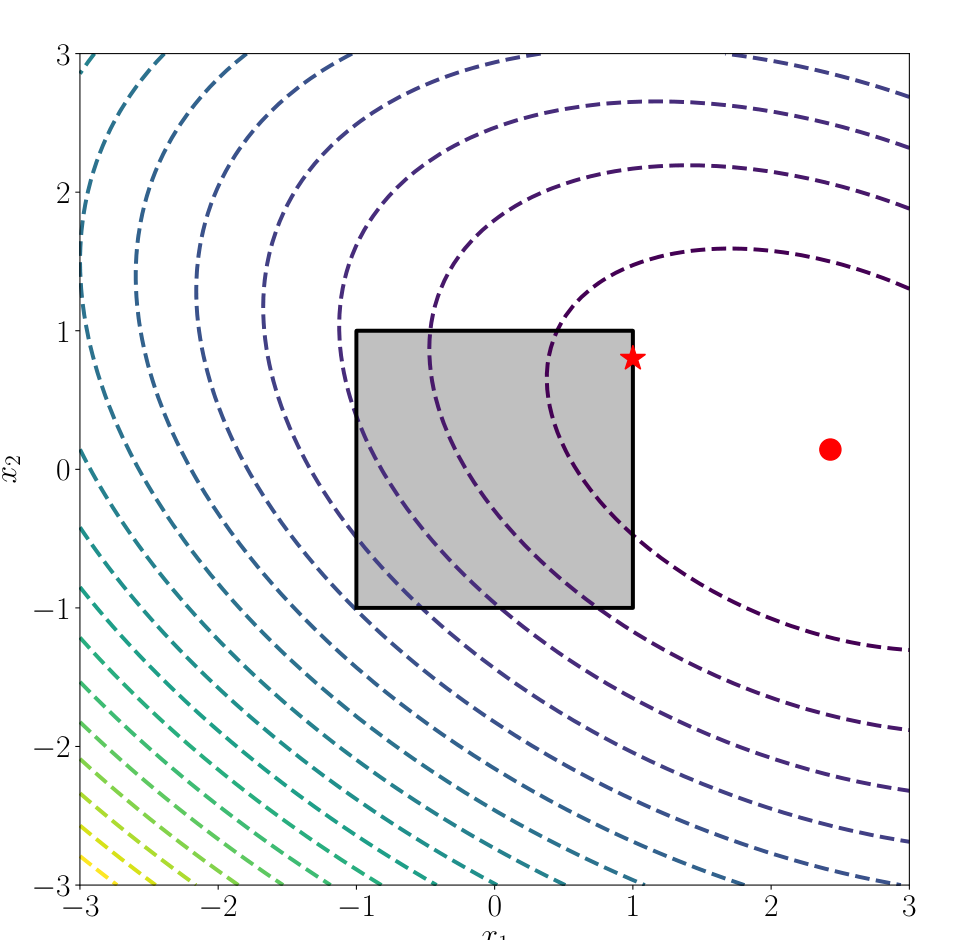
\includegraphics[width=320pt,keepaspectratio]{docs/images/Figure7.4.png}
\caption*{\refstepcounter{figcounter}\label{fig:7-4}图~\thefigcounter 带约束优化示意图。}
\end{figure}


值得指出的是，在一般情况下，函数 $ f $ 和 $ g_i $ 可能是非凸的，我们将在下一节中讨论凸的情形。

将带约束问题 (7.17) 转化为无约束问题的一种显而易见但不太实用的方法是使用 \emph{示性函数（indicator function）} ：

\begin{equation}
J(\boldsymbol{x}) = f(\boldsymbol{x}) + \sum_{i=1}^m \mathbf{1}(g_i(\boldsymbol{x}))
\tag{7.18}\label{eq:7-18}
\end{equation}

其中 $ \mathbf{1}(z) $ 是一个无穷阶跃函数：

\begin{equation}
\mathbf{1}(z) = \begin{cases} 0 & \textcn{若 } z \leqslant 0 \\ \infty & \textcn{其他} \end{cases} \textcn{。}
\tag{7.19}\label{eq:7-19}
\end{equation}

当约束不满足时，该函数会施加无穷大的惩罚，因此能够提供与原问题相同的解。然而，这个无穷阶跃函数在优化上同样极其困难。我们可以通过引入 \emph{拉格朗日乘子（Lagrange multiplier）} 来克服这一困难。拉格朗日乘子的核心思想是用线性函数来替代该阶跃函数。

通过分别为每个不等式约束引入拉格朗日乘子 $ \lambda_i \geqslant 0 $（Boyd and Vandenberghe, 2004, chapter 4），我们将问题 (7.17) 与 \emph{拉格朗日函数（Lagrangian）} 联系起来，使得：

\begin{equation}
\mathfrak{L}(\boldsymbol{x}, \boldsymbol{\lambda}) = f(\boldsymbol{x}) + \sum_{i=1}^m \lambda_i g_i(\boldsymbol{x})
\tag{7.20a}\label{eq:7-20a}
\end{equation}

\begin{equation}
= f(\boldsymbol{x}) + \boldsymbol{\lambda}^\top \boldsymbol{g}(\boldsymbol{x})
\tag{7.20b}\label{eq:7-20b}
\end{equation}

在最后一行中，我们将所有约束 $ g_i(\boldsymbol{x}) $ 拼接成向量 $ \boldsymbol{g}(\boldsymbol{x}) $，并将所有拉格朗日乘子拼接成向量 $ \boldsymbol{\lambda} \in \mathbb{R}^m $。

现在我们引入拉格朗日对偶的思想。一般而言，优化中的对偶性是指将一组变量 $ \boldsymbol{x} $（称为 \emph{原变量（primal variables）} ）的优化问题，转化为另一组不同变量 $ \boldsymbol{\lambda} $（称为 \emph{对偶变量（dual variables）} ）的优化问题。我们介绍两种不同的对偶途径：在本节中，我们讨论 \emph{拉格朗日对偶（Lagrangian duality）} ；在第 7.3.3 节中，我们将讨论 \emph{勒让德-芬歇尔对偶（Legendre–Fenchel duality）} 。

\textbf{定义 7.1}。式~\eqref{eq:7-17} 中的问题：

\begin{equation}
\begin{aligned}
\min_{\boldsymbol{x}} & \quad f(\boldsymbol{x}) \\
\text{subject to} & \quad g_i(\boldsymbol{x}) \leqslant 0 \quad \textcn{对所有 } i = 1, \ldots, m
\end{aligned}
\tag{7.21}\label{eq:7-21}
\end{equation}

被称为 \emph{原问题（primal problem）} ，对应于原变量 $ \boldsymbol{x} $。 其相应的 \emph{拉格朗日对偶问题（Lagrangian dual problem）} 由下式给出：

\begin{equation}
\begin{aligned}
\max_{\boldsymbol{\lambda} \in \mathbb{R}^m} & \quad \mathfrak{D}(\boldsymbol{\lambda}) \\
\text{subject to} & \quad \boldsymbol{\lambda} \geqslant \boldsymbol{0} ,
\end{aligned}
\tag{7.22}\label{eq:7-22}
\end{equation}

其中 $ \boldsymbol{\lambda} $ 是对偶变量，且 $ \mathfrak{D}(\boldsymbol{\lambda}) = \min_{\boldsymbol{x} \in \mathbb{R}^d} \mathfrak{L}(\boldsymbol{x}, \boldsymbol{\lambda}) $。

\emph{备注} 。在定义 7.1 的讨论中，我们使用了两个同样具有独立重要意义的概念（Boyd and Vandenberghe, 2004）。

首先是 \emph{极小极大不等式（minimax inequality）} ，它指出对于任意具有两个参数的函数 $ \phi(\boldsymbol{x}, \boldsymbol{y}) $，先极小后极大（maximin）小于等于先极大后极小（minimax），即：

\begin{equation}
\max_{\boldsymbol{y}} \min_{\boldsymbol{x}} \phi(\boldsymbol{x}, \boldsymbol{y}) \leqslant \min_{\boldsymbol{x}} \max_{\boldsymbol{y}} \phi(\boldsymbol{x}, \boldsymbol{y}) \textcn{。}
\tag{7.23}\label{eq:7-23}
\end{equation}

该不等式可以通过考虑以下不等式来证明：

\begin{equation}
\textcn{对所有 } \boldsymbol{x}, \boldsymbol{y} , \quad \min_{\boldsymbol{x}} \phi(\boldsymbol{x}, \boldsymbol{y}) \leqslant \max_{\boldsymbol{y}} \phi(\boldsymbol{x}, \boldsymbol{y}) \textcn{。}
\tag{7.24}\label{eq:7-24}
\end{equation}

注意到对式~\eqref{eq:7-24} 的左侧关于 $ \boldsymbol{y} $ 取极大值仍然保持不等式成立，因为该不等式对所有 $ \boldsymbol{y} $ 均成立。类似地，我们可以对式~\eqref{eq:7-24} 的右侧关于 $ \boldsymbol{x} $ 取极小值，从而得到式~\eqref{eq:7-23}。

第二个概念是 \emph{弱对偶性（weak duality）} ，它利用式~\eqref{eq:7-23} 证明了原问题的值始终大于或等于对偶问题的值。这在式~\eqref{eq:7-27} 中有更详细的描述。♦

回想一下，式~\eqref{eq:7-18} 中的 $ J(\boldsymbol{x}) $ 与式~\eqref{eq:7-20b} 中的拉格朗日函数之间的区别在于，我们将示性函数松弛为了线性函数。因此，当 $ \boldsymbol{\lambda} \geqslant \boldsymbol{0} $ 时，拉格朗日函数 $ \mathfrak{L}(\boldsymbol{x}, \boldsymbol{\lambda}) $ 是 $ J(\boldsymbol{x}) $ 的下界。因此，$ \mathfrak{L}(\boldsymbol{x}, \boldsymbol{\lambda}) $ 关于 $ \boldsymbol{\lambda} $ 的极大值为：

\begin{equation}
J(\boldsymbol{x}) = \max_{\boldsymbol{\lambda} \geqslant \boldsymbol{0}} \mathfrak{L}(\boldsymbol{x}, \boldsymbol{\lambda}) \textcn{。}
\tag{7.25}\label{eq:7-25}
\end{equation}

回想一下，原始问题是极小化 $ J(\boldsymbol{x}) $：

\begin{equation}
\min_{\boldsymbol{x} \in \mathbb{R}^d} \max_{\boldsymbol{\lambda} \geqslant \boldsymbol{0}} \mathfrak{L}(\boldsymbol{x}, \boldsymbol{\lambda}) \textcn{。}
\tag{7.26}\label{eq:7-26}
\end{equation}

根据极小极大不等式~\eqref{eq:7-23}，交换极小与极大的顺序会产生一个较小的值，即：

\begin{equation}
\begin{adjustbox}{max width=\linewidth}
\min_{\boldsymbol{x} \in \mathbb{R}^d} \max_{\boldsymbol{\lambda} \geqslant \boldsymbol{0}} \mathfrak{L}(\boldsymbol{x}, \boldsymbol{\lambda}) \geqslant \max_{\boldsymbol{\lambda} \geqslant \boldsymbol{0}} \min_{\boldsymbol{x} \in \mathbb{R}^d} \mathfrak{L}(\boldsymbol{x}, \boldsymbol{\lambda}) \textcn{。}
\end{adjustbox}
\tag{7.27}\label{eq:7-27}
\end{equation}

这也称为 \emph{弱对偶性（weak duality）} 。注意到右侧的内部部分正是 \emph{对偶目标函数（dual objective function）} $ \mathfrak{D}(\boldsymbol{\lambda}) $，定义由此自然得出。

与带有约束的原始优化问题相比，对于给定的 $ \boldsymbol{\lambda} $ 值，$ \min_{\boldsymbol{x} \in \mathbb{R}^d} \mathfrak{L}(\boldsymbol{x}, \boldsymbol{\lambda}) $ 是一个无约束优化问题。如果求解 $ \min_{\boldsymbol{x} \in \mathbb{R}^d} \mathfrak{L}(\boldsymbol{x}, \boldsymbol{\lambda}) $ 很简单，那么整个问题就容易求解。原因在于外层问题（关于 $ \boldsymbol{\lambda} $ 的极大化）是一组仿射函数的逐点极大值，因此即便 $ f(\cdot) $ 和 $ g_i(\cdot) $ 可能非凸，它也是一个凹函数。凹函数的极大值可以被高效地计算。

假定 $ f(\cdot) $ 和 $ g_i(\cdot) $ 是可微的，我们通过对拉格朗日函数关于 $ \boldsymbol{x} $ 求微分，令微分（导数）为零，并解出最优值，从而求得拉格朗日对偶问题。我们将在第 7.3.1 节和第 7.3.2 节中讨论两个具体示例，其中 $ f(\cdot) $ 和 $ g_i(\cdot) $ 均是凸的。

\emph{备注} （等式约束）。考虑式~\eqref{eq:7-17} 带有额外等式约束的情形：

\begin{equation}
\begin{adjustbox}{max width=\linewidth}
\begin{aligned}
\min_{\boldsymbol{x}} & \quad f(\boldsymbol{x}) \\
\text{subject to} & \quad g_i(\boldsymbol{x}) \leqslant 0 \quad \textcn{对所有 } i = 1, \ldots, m \\
& \quad h_j(\boldsymbol{x}) = 0 \quad \textcn{对所有 } j = 1, \ldots, n \textcn{。}
\end{aligned}
\end{adjustbox}
\tag{7.28}\label{eq:7-28}
\end{equation}

我们可以通过将等式约束替换为两个不等式约束来对其进行建模。也就是说，对于每个等式约束 $ h_j(\boldsymbol{x}) = 0 $，我们将其等价替换为两个约束 $ h_j(\boldsymbol{x}) \leqslant 0 $ 和 $ h_j(\boldsymbol{x}) \geqslant 0 $。事实证明，由此得到的拉格朗日乘子是不受约束的。

因此，我们对式~\eqref{eq:7-28} 中对应于不等式约束的拉格朗日乘子施加非负约束，而对应于等式约束的拉格朗日乘子则不受约束。♦
